The first four conditions describe the stages before CPU prefetch was added to video extraction. They were measured on the AMD RX~9070~XT. Video times include model loading; text and audio times exclude loading. The samples contain 32 video clips, 128 words, and four 60-second audio events. Each modality is a separate workload; these speed ratios do not measure a combined pipeline. Table~\ref{tab:features-performance} reports medians and ratios; Table~\ref{tab:features-raw} retains both repetitions. No confidence intervals are claimed.

\begin{table}[htbp]\centering\sffamily\small
\caption{Before video prefetch: median extraction time and peak GPU tensor allocation across two repetitions per condition. Speedup is original/candidate median; peak allocation is the maximum across repetitions. Video times include load; text and audio exclude load. *Video FP16 uses a separately recorded FP32 video baseline and is not interleaved with the FP16 runs.}\label{tab:features-performance}
\begin{tabular}{@{}lrrrrr@{}}\toprule
Condition & Orig. (s) & New (s) & Speedup & Orig. (GiB) & New (GiB) \\\midrule
Video FP32 & 242.102 & 197.060 & 1.23 & 9.468 & 4.517 \\
Video FP16* & 242.102 & 21.182 & 11.43 & 9.468 & 2.257 \\
Text BF16 & 14.265 & 6.289 & 2.27 & 7.530 & 7.039 \\
Audio FP32 & 4.638 & 4.085 & 1.14 & 7.464 & 7.464 \\
\bottomrule\end{tabular}\end{table}

\begin{table}[htbp]\centering\sffamily\small
\caption{Before video prefetch: raw extraction times (s). Video FP32 and FP16 are not interleaved; the FP16 candidate is compared against the separately recorded FP32 baseline median.}\label{tab:features-raw}
\begin{tabular}{@{}lrr@{}}\toprule
Condition & Original repetitions (s) & Candidate repetitions (s) \\\midrule
Video FP32 & 241.809, 242.395 & 197.043, 197.076 \\
Text BF16 & 13.049, 15.481 & 6.269, 6.308 \\
Audio FP32 & 4.670, 4.605 & 4.081, 4.090 \\
Video FP16* & 241.809, 242.395 & 21.358, 21.006 \\
\bottomrule\end{tabular}\end{table}

Figure~\ref{fig:features-performance} shows normalized extraction time with the original as 1 and the peak GPU tensor allocation. Candidate repetitions appear as points. FP16 changes feature values, so downstream score margins determine its acceptance.

Figure~\ref{fig:features-accuracy} reports score drift over all 168 existing subjects. The worst subject/movie pair determines acceptance; averaging subjects cannot hide a failure. The initial single-subject alignment check is retained in Table~\ref{tab:features-accuracy}.

\begin{table}[htbp]\centering\sffamily\small
\caption{Existing-subject brain-score agreement for the FP16 video path. Baseline and candidate mean parcel correlations are shown to six decimals; deltas use scientific notation. Margins: mean $|\Delta r| \leq 10^{-4}$, max parcel $|\Delta r| \leq 10^{-3}$, $|\Delta \mathrm{MSE}|/\mathrm{MSE} \leq 10^{-3}$.}\label{tab:features-accuracy}
\begin{tabular}{@{}lrrrrr@{}}\toprule
Movie & Orig. mean $r$ & New mean $r$ & $\Delta$ mean $r$ & Max $|\Delta r|$ & Rel. MSE \\\midrule
Movie 1 & 0.236518 & 0.236493 & $-2.49\times10^{-5}$ & $3.80\times10^{-4}$ & $1.62\times10^{-6}$ \\
Movie 2 & 0.263297 & 0.263328 & $3.15\times10^{-5}$ & $2.74\times10^{-4}$ & $-8.88\times10^{-6}$ \\
Movie 3 & 0.200522 & 0.200527 & $4.67\times10^{-6}$ & $3.81\times10^{-4}$ & $-3.67\times10^{-6}$ \\
Movie 4 & 0.257067 & 0.257074 & $6.19\times10^{-6}$ & $2.87\times10^{-4}$ & $-5.39\times10^{-6}$ \\
\bottomrule\end{tabular}\end{table}

4 of four movies satisfy all three prespecified margins. These are engineering margins, not statistical equivalence tests.

\begin{table}[htbp]\centering\sffamily\small
\caption{FP16 regression across all 168 existing subjects per movie. Worst changes take the maximum absolute change across subjects (and parcels for parcel r); each subject/movie pair uses the fixed margins.}\label{tab:cohort}
\begin{tabular}{@{}lrrrrr@{}}\toprule
Movie & Orig. mean $r$ & New mean $r$ & Max $|\Delta\bar r|$ & Max $|\Delta r|$ & Max rel. $|\Delta$MSE$|$ \\\midrule
1 & 0.207309 & 0.207298 & $6.51\times10^{-5}$ & $7.08\times10^{-4}$ & $2.21\times10^{-5}$ \\
2 & 0.227327 & 0.227322 & $6.32\times10^{-5}$ & $4.21\times10^{-4}$ & $1.65\times10^{-5}$ \\
3 & 0.207018 & 0.207009 & $5.46\times10^{-5}$ & $7.88\times10^{-4}$ & $3.19\times10^{-5}$ \\
4 & 0.240679 & 0.240680 & $3.25\times10^{-5}$ & $4.23\times10^{-4}$ & $1.58\times10^{-5}$ \\
\bottomrule\end{tabular}\end{table}

Table~\ref{tab:cohort} covers all 672 subject/movie pairs; 0 exceed at least one margin. The cohort is an existing cache, not an independently held-out population. No participant identifiers or individual diagnostic rows are redistributed.

\begin{figure}[htbp]\centering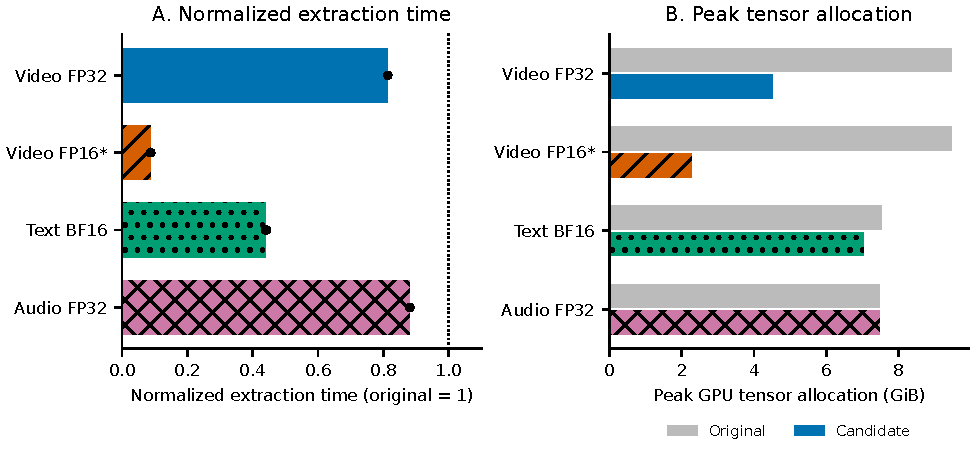
\includegraphics[width=\linewidth]{features-performance.pdf}\caption{Extraction costs before video prefetch. Left: bars show candidate/original median time; black points show the two candidate repetitions divided by the original median. Right: gray and colored bars show original and candidate peak GPU tensor allocation, respectively, taking the maximum of two runs. Video FP16 (*) was timed separately from the original FP32 runs. Allocation excludes non-PyTorch VRAM.}\label{fig:features-performance}\end{figure}

\begin{figure}[htbp]\centering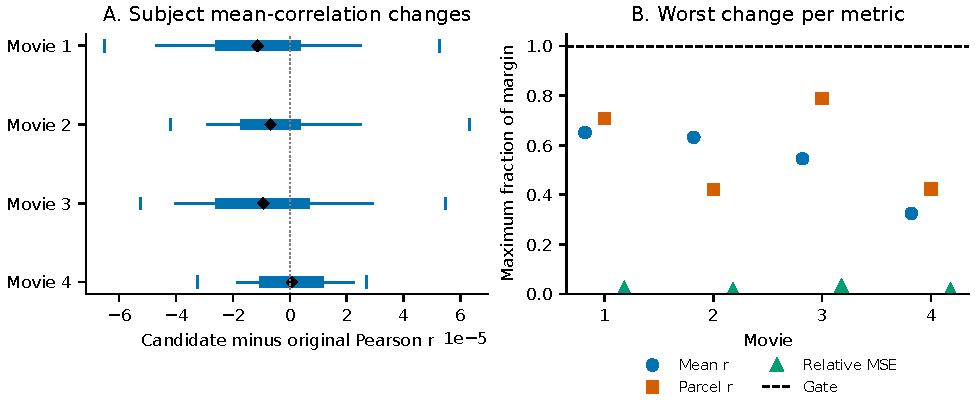
\includegraphics[width=\linewidth]{features-accuracy.pdf}\caption{Serial float16 video regression on four movies across 168 existing subjects. Left: diamonds, subject median change in mean parcel r; thick lines, interquartile range; thin lines, 5th--95th percentiles; ticks, extrema. These are subject distributions, not confidence intervals. Right: the maximum for each metric divided by its fixed margin; these maxima may come from different subjects. Circles show mean r, squares maximum parcel r, and triangles relative labeled-vertex MSE. Values at or below 1 pass.}\label{fig:features-accuracy}\end{figure}

\subsection{Final video path with CPU prefetch}

The final path overlaps one CPU frame window with GPU inference. Table~\ref{tab:prefetch-long} compares it with serial FP16 on one 60-second event. All three pairs are finite and bitwise equal over 3,379,200 values per pair. The 168-subject precision evaluation used the serial FP16 path; the full cohort was not re-extracted with prefetch. The separate prefetch check covers these 120 clips.

\begin{table}[htbp]\centering\sffamily\small
\caption{Production prefetch: three alternating pairs on one 60-second event; loading included. Serial control performs the same CPU reads when the main thread requests each result.}\label{tab:prefetch-long}
\begin{tabular}{@{}lrr@{}}\toprule
Pair & Serial FP16 (s) & Prefetch FP16 (s) \\\midrule
1 & 74.334 & 69.814 \\
2 & 75.736 & 69.899 \\
3 & 75.503 & 70.282 \\
Median & 75.503 & 69.899 \\
\bottomrule\end{tabular}\end{table}

The median reduction is 7.42\%. One future bounds CPU lookahead to one window; GPU inference stays on the main thread. The worker is joined before the video reader closes, including on inference errors.

\begin{table}[htbp]\centering\sffamily\small
\caption{Final short-event extraction: 32 clips, two repetitions, model loading included. The original FP32 baseline was recorded separately; these conditions were not interleaved.}\label{tab:prefetch-short}
\begin{tabular}{@{}lrrr@{}}\toprule
Condition & Median (s) & Speedup & Peak (GiB) \\\midrule
Original FP32 & 242.102 & 1.00 & 9.468 \\
FP16 with prefetch & 20.051 & 12.07 & 2.257 \\
\bottomrule\end{tabular}\end{table}

The final short-event repetitions took 19.995, 20.106 s. The short-event and 60-second workloads differ; their speed ratios are not multiplied.
